%% ------------------------------------------------------------------------- %%
\chapter{Telas OLED Flexíveis}
\label{cap:oled}

A tecnologia OLED é baseada na iluminação através da aplicação de eletricidade em moléculas organicas \cite{HSWOLED}, denominado \bf{eletroluminescência}, como mostra a imagem \ref{fig:oled_early_product}. A \bf{eletroluminescência} foi inicialmente pesquisada por André Bernanose e colegas de trabalho em 1950 na Nancy-Université na França. Eles aplicaram alta tensão (AC) no ar para materias como a \bf{acridina laranja}, depositada e dissolvida em filmes finos de celulose ou celofane. O mecanismo proposto era a excitação direta das moléculas do corante ou a excitação de seus elétrons \cite{WikipediaOLED}.

Em 1960, Martin Pope e colaboradores da Universidade de Nova York desenvolveram eletrodos injetáveis óhmicos de contato a partir de cristais orgânicos. Eles descreveram ainda os requisitos energéticos necessários (funções trabalho) para os eletrodos de contato injetados. Esses contatos são a base da injeção de carga em todos os dispositivos OLED modernos. O grupo de Pope também observou pela primeira vez \bf{eletroluminescência} de corrente contínua (DC) sob vácuo em um único cristal puro de antraceno e em cristais de antraceno embebidos com tetraceno em 1963, usando uma pequena área de eletrodo de prata em 400V. \cite{WikipediaOLED}

\begin{figure}[!h]
  \centering
  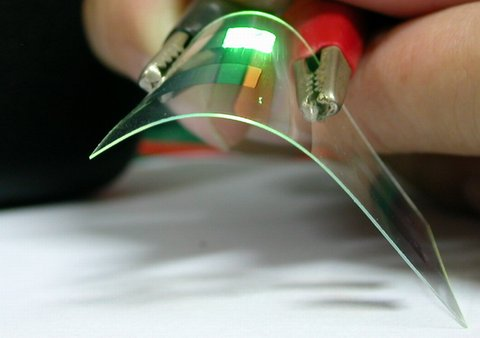
\includegraphics[width=.40\textwidth]{oled_early_product} 
  \caption{Uma tela flexível OLED}
  \label{fig:oled_early_product} 
\end{figure}

OLED's são dispositivos solidos compostos composto por finas camadas de moléculas organicas que são capazes de criar eletricidade através da aplicação de eletricidade. OLED's podem prover imagens mais brilhantes, maior nitidez e consumindo menos elergia que suas antecessoras, LCD e LED \cite{HSWOLED}.

O OLED é um dispositivo semi-condutor sólido de 100 a 500 nanometros de espessura, ou seja, aproximadamente 200 vezes mais fino que um fio de cabelo humano. OLED's podem ter de 2 a 3 camadas de material orgânico; sendo que a terceira camada ajuda no transporte de elétron do cátodo para a camada emissiva \ref{fig:camadas_oled} \cite{HSWOLED}.

%% ------------------------------------------------------------------------- %%
\section{Origem}
\label{sec:camadas}

Dr. Ching Tang e Steven Van Slyke são os dois pioneiros da tecnologia OLED - de fato podemos dizer que eles são os inventores da tecnologia OLED em 1987 na Eastman Kodak. Os dois escreveram o artigo \textit{Electroluminescent devices with improved cathodes} para um seminário e este tem sido citado em mais de 5000 publicações. Agora, os dois pioneiros foram incluidos no \textit{hall} da fama dos consumidores de eletronicos \cite{OLEDPioneers}. 

\begin{figure}[!h]
  \centering
  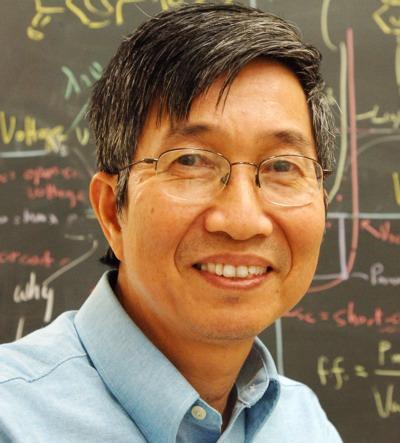
\includegraphics[width=.40\textwidth]{ching_tang} 
  \caption{Criador da tecnologia OLED Ching Tang}
  \label{fig:ching_tang} 
\end{figure}

\begin{figure}[!h]
  \centering
  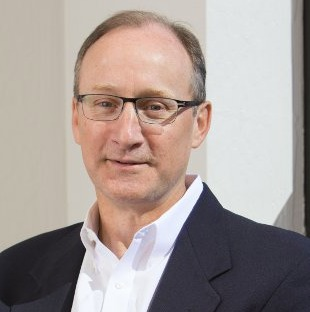
\includegraphics[width=.40\textwidth]{steven_slyke} 
  \caption{Criador da tecnologia OLED Steven Van Slyke}
  \label{fig:steven_slyke} 
\end{figure}


%% ------------------------------------------------------------------------- %%
\section{Vantagens}
\label{sec:vantagens}


%% ------------------------------------------------------------------------- %%
\section{Composição e Criação}
\label{sec:camadas}

\begin{figure}[!h]
  \centering
  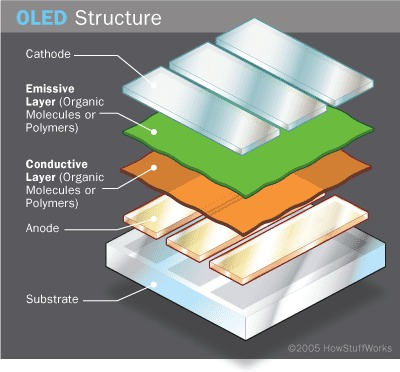
\includegraphics[width=.40\textwidth]{camadas_oled} 
  \caption{Componentes OLED}
  \label{fig:camadas_oled} 
\end{figure}


%% ------------------------------------------------------------------------- %%
\subsection{Substrato (\textit{Substrate})}
\label{sec:substrato}

Produzido a partir de plástico transparente, vidro ou folha metálica possui a função de suportar o OLED.


%% ------------------------------------------------------------------------- %%
\subsection{Anódio (\textit{Anode})}
\label{sec:substrato}

Sendo transparente, o anódio remove elétrons, ou seja, adiciona "buracos" de elétrons, enquanto há corrente elétrica no dispositivo.


%% ------------------------------------------------------------------------- %%
\subsection{Camadas Orgânicas (\textit{Organic layers})}
\label{sec:substrato}

Estas camadas são feitas de moléculas organicas ou polímeros, sendo que os tipos de moléculas e polímeros são diferentes entre as camadas.

\bf{Camada Condutiva:} Esta camada é feita de moléculas orgânicas plásticas que transportam os "buracos" do Anódio. Um polímero usado nesta camada é a polianilina.

\bf{Camada Emissiva:} Esta camada é feira de moléculas orgânicas plásticas, diferentes da camada Condutiva, e transporta elétrons do Catódio. É nesta camada onde a luz é gerada. Um dos polímeros usados nesta camada é o polifluoreno. 


%% ------------------------------------------------------------------------- %%
\subsection{Catódio (\textit{Cathode})}
\label{sec:substrato}

Pode ser ou não transparente, a depender do tipo de OLED. Esta camada injeta elétrons enquanto a corrente elétrica flui através do dispositivo. 

O maior trabalho na construção de uma tela OLED é aplicar a camada orgânica ao substrato. Existem três maneiras de se fazer isso:

\begin{enumerate}
\item \bf{Deposição a vácuo ou evaporação térmica a vácuo:} Em uma câmera de vácuo, as moléculas orgânicas são aquecidas suavemente (evaporadas) e é condensada como finas camadas sobre o substrato arrefecido. Este processo é caro e ineficiente.

\item \bf{Deposição de vapor orgânico em fase:} Em uma de baixa pressão, câmara do reator quente de paredes, um transporte de gás portador evaporado moléculas orgânicas sobre substratos resfriados, onde se condensam em filmes finos. Utilizando um gás transportador aumenta a eficiência e reduz o custo de fabricação de OLEDs.
\item 
\item 
\end{enumerate}



Inkjet printing - With inkjet technology, OLEDs are sprayed onto substrates just like inks are sprayed onto paper during printing. Inkjet technology greatly reduces the cost of OLED manufacturing and allows OLEDs to be printed onto very large films for large displays like 80-inch TV screens or electronic billboards.


%% ------------------------------------------------------------------------- %%
\section{Funcionamento}
\label{sec:funcionamento}


%% ------------------------------------------------------------------------- %%
\section{Produto}
\label{sec:funcionamento}